\subsection{Normalized Angular Velocity Input}
In the steady-state condition ($\dot \omega = 0$), (\ref{eqn::dyn_mdl}) simplifies to:
%===
\begin{align}
    &\frac{b_m}{K_r} \left(\frac{\omega_m}{V_{in}}\right) + \frac{V_{in}}{K_r} C_D \lr{\frac{\omega}{V_{in}}}^2 + \frac{M_f}{K_r V_{in}} = u_m
\end{align}
%===
We introduce a term, $u_{\omega}$, which represents the angular velocity of the motor with the propeller at unit supply voltage for the given PWM input ($u_p$). This is termed as "\textit{Normalized Angular Velocity}".
%===
\begin{align}
    u_{\omega} &= \frac{\omega}{V_{in}} \text{  at  } u_m = g_m(u_p) \\
    %===
    \implies u_m &= \underbrace{\frac{b_m}{K_r} u_\omega + \frac{\hat V_{in}}{K_r} C_D u_\omega^2 + \frac{M_f}{K_r  \hat V_{in}}}_{g_\omega (u_\omega, \hat V_{in})}
     \label{eqn::input_def}
\end{align}
where $\hat V_{in}$ is the battery voltage at calibration $(15.54\,V)$.
%===
The relationship between $u_\omega$ and $u_p$ can be estimated from the static
measurement data (Fig.-\ref{fig::norm_omega}).
%===
\begin{figure}[h]
    \centering
    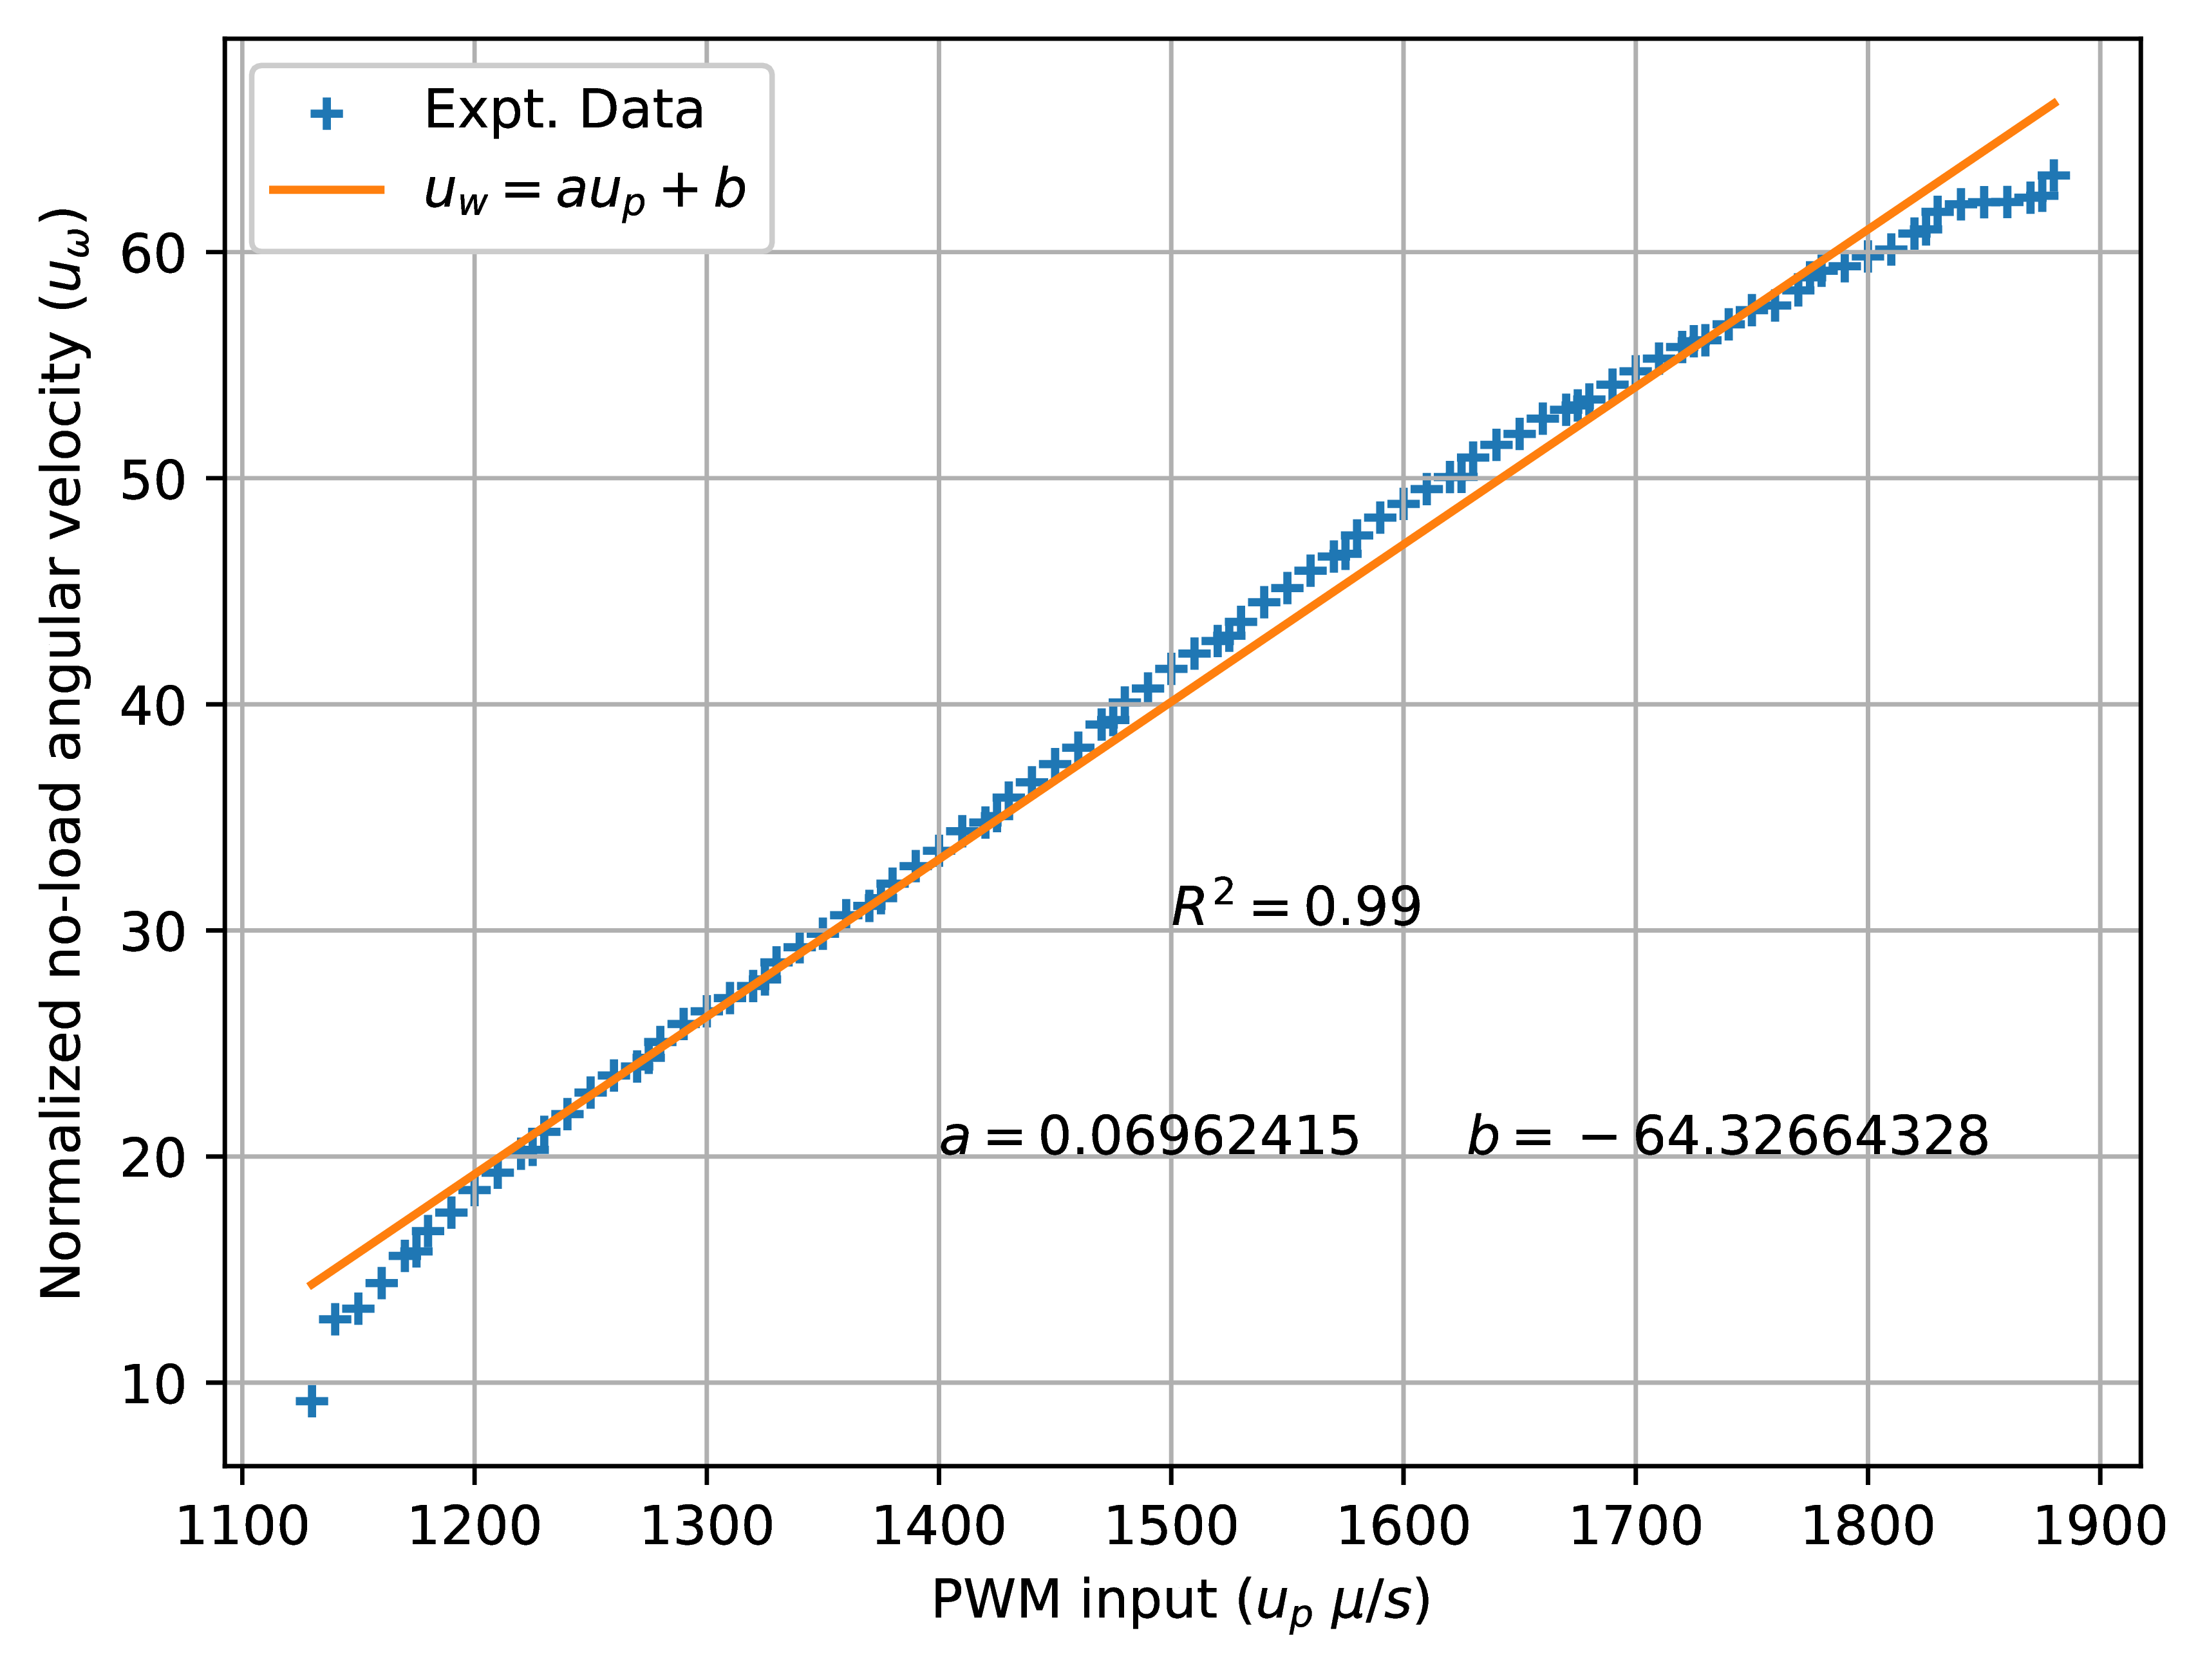
\includegraphics[width = \figsize]{./figs/figs_acc/norm_omega/no-load_rpm.png}
    \caption{$u_\omega$ as a function of $u_p$}
    \label{fig::norm_omega}
\end{figure}
%===
\begin{align}
    &u_\omega = a u_p + b
    \quad a = 0.0696
    \quad b = -64.3266   \label{eqn::uw_calib}\\
    \implies& g_m(u_p) = g_\omega(a u_p  + b, \hat V_{in})
    \; [\because u_m = g_\omega(u_\omega, \hat V_{in})]
\end{align}
